\chapter{Exploración}%
\label{cha:exploración}

\lecture{18}{2020-07-14}{Exploration (Part 1)}

\section{¿Qué es la exploración? ¿Por qué es un problema?}%
\label{sec:_qué_es_la_exploración_por_qué_es_un_problema_}

Desde el punto de vista del algoritmo no se conocen las reglas del entorno en el que se tiene
que desenvolver. Solo recibe las señales de recompensa y a partir de eso tiene que averiguar
que es lo que está bien y que es lo que está mal, por lo que va descubriendo las reglas a partir
de prueba y error. Descubrir las reglas es de notoria dificultad si las tareas se extienden
en el tiempo como por ejemplo en Montezuma's Revenge.

Dos posibles definiciones para el problema de la exploración son:
\begin{itemize}
    \item ¿Cómo puede un agente descubrir estrategias que den na alta recompensa que
        requieran de una secuencia compleja de acciones extendida en el tiempo que,
        individualmente, no devuelven una recompensa?
    \item ¿Cómo puede un agente decidir si probar nuevos comportamientos (descubrir nuevos
        con mejores recompensas) o continuar haciendo la mejor acción conocida hasta el
        momento?
\end{itemize}

En realidad es el mismo problema, en el que se tiene que balancear entre:
\begin{itemize}
    \item Explotación: hacer lo que se 'sabe' que va a dar la mayor recompensa.
    \item Exploración: hacer cosas que no se han probado antes con la intención de
        encontrar recompensas mayores.
\end{itemize}

La exploración es un problema complicado.

\begin{center}
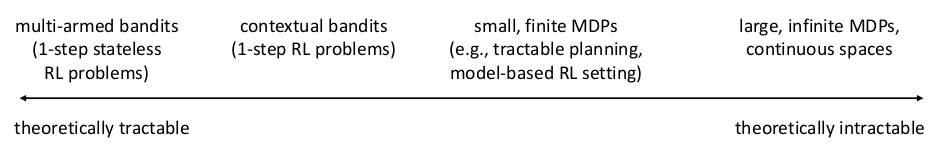
\includegraphics[width=0.8\textwidth]{figures/2020-07-14-165551_940x151_scrot.png}
\end{center}

Se puede formalizar el proceso de exploración como la identificación de un POMDP. El
aprendizaje de la política es trivial incluso en POMDP. 

\section{\textit{Multi-armed bandits}}%
\label{sec:multi-armed bandits}

En un problema de múltiples bandidos (máquinas tragaperras), el espacio de acciones es
$A=\{pull_1, pull_2,\ldots,pull_n\}$. Se quiere encontrar que acciones llevan a la máxima
recompensa, ya que ciertas máquinas dan más dinero que otras. Se puede asumir que
$r(a_n)\sim p(r|a_n)$. 

Un bandido se define como $r(a_i)\sim p_{\theta_i}(r_i)$. Por ejemplo  $p(r_i=1)=\theta_i$
y  $p(r_i=0)=1-\theta_i$. Se asume que puede haber un prior, pero de otra forma son
desconocidos.

Esto define un POMDP con  $s=[\theta_1,\ldots,\theta_n]$. Los estados son las probabilidades
que se piensa que se tienen en todos los bandidos. 

Se necesita una medida de como de bien se está haciendo la exploración, esta medida se le llama
arrepentimiento (\textit{regret}) y mide la diferencia con respecto a la política óptima en
el paso $T$.
\begin{align}
    Reg(T)=TE[r(a^*)]-\sum_{t=1}^T r(a_t)
\end{align}
No es una medida que se pueda usar en un problema que se tenga que resolver, pero sirve para
comparar entre varios algoritmos.

Hay varias estrategias simples para 'vencer' el problema de los bandidos. Típicamente lo que
se quiere es demostrar una cota del arrepentimiento en la esperanza. Hay varios algoritmos
que son igual de óptimos hasta un factor constante, y varían muy poco entre ellos dependiendo
del problema. 

La exploración basada en métodos más complicados como DRL carece de las garantías de
convergencia de los métodos sencillos.

\section{Exploración basada en optimismo}%
\label{sec:exploración_basada_en_optimismo}

Es una de la más sencillas pero de las más efectivas. Se tiene en cuenta la media de las
recompensas $\hat{\mu}_a$ para cada acción $a$. De modo que la explotación queda en elegir
$a=arg\max \hat{\mu}_a$. Esto no se quiere hacer siempre ya que no se explorará.

En vez de coger el máximo siempre, se va a bonificar a las acciones que se hayan cogido pocas
veces:
\begin{align}
    a=arg\max \hat{\mu}_a+C\sigma_a
\end{align}

Hay muchas formas de elegir $\sigma$. Una regla UCB bastante buena es (Auer et al.):
\begin{align}
    a=arg\max \hat{\mu}_a + \sqrt{ \frac{2\log T}{N(a)}  }
\end{align}

Con esto Reg(T) es $O(\log T)$, que está demostrado que es lo mejor que se puede obtener.

\section{Posterior matching exploration}%
\label{sec:posterior_matching_exploration}

Se asume que $r(a_i)\sim p_{\theta_i}(r_i)$. Se define un POMDP como
$s=[\theta_1,\ldots,\theta_n]$. El estado de creencias es $\hat{p}(\theta_1,\ldots,\theta_n)$.

La idea es simple, se supone que nuestras creencias $\hat{p}$ son correctas y se actúa con
respecto a ellas. Naturalmente se tiene una fuerte exploración. Una vez se ha tomado la acción,
se mira el resultado y se actualizan nuestras creencias de nuevo.

Es más difícil de analizar teóricamente pero empíricamente funciona muy bien.

\section{Information-theoretic exploration}%
\label{sec:information_theoretic_exploration}

Está basado en la ganancia de información, por lo que necesita un poco más de explicación.

Diseño experimental Bayesiano: se quiere determinar una variable latente $z$ (por ejemplo $z$
puede ser la acción óptima o su valor).  $H(\hat{p}(z))$ es la entropía de nuestra estimación
de $z$. $H(\hat{p}(z)|y)$ es la entropía de nuestra estimación de $z$ después de observar
$z$ (por ejemplo $y$ puede ser $r(a)$). Se define la ganancia de información como:
\begin{align}
    IG(z,y)=E_y[H(\hat{p}(z))-H(\hat{p}(z)|y)]
\end{align}

Normalmente depende de las acciones por lo que se tiene $IG(z,y|a)$. Por lo que para estimar
mejor  $z$ se tiene que coger $a$ que de la mayor ganancia de información.

\section{Métodos de exploración en DRL}%
\label{sec:métodos_de_exploración_en_drl}

\subsubsection{Exploración optimista}%
\label{ssub:exploración_optimista}

La función de bonus de exploración pueden ser muchas, siempre que decrezcan con $N(a)$. Se puede
usar esta idea con MDP, ahora se usa  $N(s,a)$ o $N(s)$ para añadir el bonus a la exploración.
Por lo que ahora $r^+(s,a)=r(s,a)+B(N(s))$. Ahora se usa  $r^+$ en vez de $r$ con cualquier
algoritmo sin modelo.

Para casos en que los estados sean incontables (imágenes por ejemplo), es imposible e
impráctico tener una cuenta de todas las veces que han aparecido los estados. Por lo
que se puede entrenar un aproximador de funciones para que mantenga la cuenta entre estados
similares.

Se va a entrenar un modelo de densidad $p_\theta(s)$ o $p_\theta(s,a)$ que nos de un número que
sea pequeño para estados similares que no ha visto nunca y grande para estados similares que ya ha visitado. 

Si se tiene un MDP pequeño tabular, la probabilidad está relacionada con la cuenta de los
estados:
\begin{align}
    P(s)= \frac{N(s)}{n} 
\end{align}
$n$ es el número de estados vistos. Después de que se vea $s$, se actualiza como:
\begin{align}
    P'(s)= \frac{N(s)+1}{n+1} 
\end{align}
Para hacer los pseudo-contadores se ajusta $p_\theta(s)$ a todos los estados $D$ vistos hasta
ahora. Se toma un pas $i$ y se observa $s_i$. Se ajusta el nuevo modelo $p_{\theta'}(s)$ a
$D \cup s_i$. Finalmente se usa $p_\theta(s_i)$ y $p_{\theta'}(s_i)$ para estimar
$\hat{N}(s)$ y se pone $r^+_i=r_i+B(\hat{N}(s))$. 

Para conseguir $\hat{N}(s)$ se resuelve el sistema de ecuaciones formado por las dos ecuaciones
anteriores.

Otra forma de estimar las cuentas es mediante los errores. Se tiene un modelo capaz de
sobreentrenarse sobre los estados. Se entrenan para que pase por los datos visitados, por lo
que los datos que no estén visitados no pasarán por las predicciones del modelo y se puede
medir el error.

\begin{center}
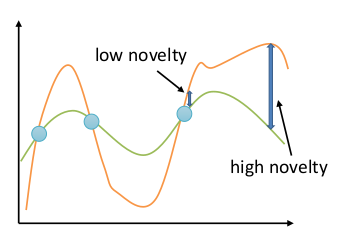
\includegraphics[width=0.5\textwidth]{figures/2020-07-14-181819_342x235_scrot.png}
\end{center}

\subsubsection{Muestreo de Thompson}%
\label{ssub:muestreo_de_thompson}

\subsubsection{Ganancia de información}%
\label{ssub:ganancia_de_información}




